%%
% Copyright (c) 2017 - 2019, Pascal Wagler;  
% Copyright (c) 2014 - 2019, John MacFarlane
% 
% All rights reserved.
% 
% Redistribution and use in source and binary forms, with or without 
% modification, are permitted provided that the following conditions 
% are met:
% 
% - Redistributions of source code must retain the above copyright 
% notice, this list of conditions and the following disclaimer.
% 
% - Redistributions in binary form must reproduce the above copyright 
% notice, this list of conditions and the following disclaimer in the 
% documentation and/or other materials provided with the distribution.
% 
% - Neither the name of John MacFarlane nor the names of other 
% contributors may be used to endorse or promote products derived 
% from this software without specific prior written permission.
% 
% THIS SOFTWARE IS PROVIDED BY THE COPYRIGHT HOLDERS AND CONTRIBUTORS 
% "AS IS" AND ANY EXPRESS OR IMPLIED WARRANTIES, INCLUDING, BUT NOT 
% LIMITED TO, THE IMPLIED WARRANTIES OF MERCHANTABILITY AND FITNESS 
% FOR A PARTICULAR PURPOSE ARE DISCLAIMED. IN NO EVENT SHALL THE 
% COPYRIGHT OWNER OR CONTRIBUTORS BE LIABLE FOR ANY DIRECT, INDIRECT, 
% INCIDENTAL, SPECIAL, EXEMPLARY, OR CONSEQUENTIAL DAMAGES (INCLUDING,
% BUT NOT LIMITED TO, PROCUREMENT OF SUBSTITUTE GOODS OR SERVICES; 
% LOSS OF USE, DATA, OR PROFITS; OR BUSINESS INTERRUPTION) HOWEVER 
% CAUSED AND ON ANY THEORY OF LIABILITY, WHETHER IN CONTRACT, STRICT 
% LIABILITY, OR TORT (INCLUDING NEGLIGENCE OR OTHERWISE) ARISING IN 
% ANY WAY OUT OF THE USE OF THIS SOFTWARE, EVEN IF ADVISED OF THE 
% POSSIBILITY OF SUCH DAMAGE.
%%

%%
% This is the Eisvogel pandoc LaTeX template.
%
% For usage information and examples visit the official GitHub page:
% https://github.com/Wandmalfarbe/pandoc-latex-template
%%

\PassOptionsToPackage{unicode=true}{hyperref} % options for packages loaded elsewhere
\PassOptionsToPackage{hyphens}{url}
\PassOptionsToPackage{dvipsnames,svgnames*,x11names*,table}{xcolor}
%
\documentclass[
  10pt,
  english,
  letterpaper,
,tablecaptionabove
]{scrartcl}
\usepackage{lmodern}
\usepackage{setspace}
\setstretch{1.2}
\usepackage{amssymb,amsmath}
\usepackage{ifxetex,ifluatex}
\ifnum 0\ifxetex 1\fi\ifluatex 1\fi=0 % if pdftex
  \usepackage[T1]{fontenc}
  \usepackage[utf8]{inputenc}
  \usepackage{textcomp} % provides euro and other symbols
\else % if luatex or xelatex
  \usepackage{unicode-math}
  \defaultfontfeatures{Scale=MatchLowercase}
  \defaultfontfeatures[\rmfamily]{Ligatures=TeX,Scale=1}
\fi
% use upquote if available, for straight quotes in verbatim environments
\IfFileExists{upquote.sty}{\usepackage{upquote}}{}
\IfFileExists{microtype.sty}{% use microtype if available
  \usepackage[]{microtype}
  \UseMicrotypeSet[protrusion]{basicmath} % disable protrusion for tt fonts
}{}
\makeatletter
\@ifundefined{KOMAClassName}{% if non-KOMA class
  \IfFileExists{parskip.sty}{%
    \usepackage{parskip}
  }{% else
    \setlength{\parindent}{0pt}
    \setlength{\parskip}{6pt plus 2pt minus 1pt}}
}{% if KOMA class
  \KOMAoptions{parskip=half}}
\makeatother
\usepackage{xcolor}
\definecolor{default-linkcolor}{HTML}{A50000}
\definecolor{default-filecolor}{HTML}{A50000}
\definecolor{default-citecolor}{HTML}{4077C0}
\definecolor{default-urlcolor}{HTML}{4077C0}
\IfFileExists{xurl.sty}{\usepackage{xurl}}{} % add URL line breaks if available
\IfFileExists{bookmark.sty}{\usepackage{bookmark}}{\usepackage{hyperref}}
\hypersetup{
  pdftitle={Hashing (Part 3)},
  pdfauthor={Connor Baker},
  pdfsubject={Hashing},
  pdfkeywords={Lecture, Hashing},
  pdfborder={0 0 0},
  breaklinks=true}
\urlstyle{same}  % don't use monospace font for urls
\usepackage[margin=2.5cm,includehead=true,includefoot=true,centering]{geometry}
\usepackage{listings}
\newcommand{\passthrough}[1]{#1}
\lstset{defaultdialect=[5.3]Lua}
\lstset{defaultdialect=[x86masm]Assembler}
\usepackage{longtable,booktabs}
% Allow footnotes in longtable head/foot
\IfFileExists{footnotehyper.sty}{\usepackage{footnotehyper}}{\usepackage{footnote}}
\makesavenoteenv{longtable}
\usepackage{graphicx,grffile}
\makeatletter
\def\maxwidth{\ifdim\Gin@nat@width>\linewidth\linewidth\else\Gin@nat@width\fi}
\def\maxheight{\ifdim\Gin@nat@height>\textheight\textheight\else\Gin@nat@height\fi}
\makeatother
% Scale images if necessary, so that they will not overflow the page
% margins by default, and it is still possible to overwrite the defaults
% using explicit options in \includegraphics[width, height, ...]{}
\setkeys{Gin}{width=\maxwidth,height=\maxheight,keepaspectratio}
\setlength{\emergencystretch}{3em}  % prevent overfull lines
\providecommand{\tightlist}{%
  \setlength{\itemsep}{0pt}\setlength{\parskip}{0pt}}
\setcounter{secnumdepth}{-\maxdimen} % remove section numbering
% Redefines (sub)paragraphs to behave more like sections
\ifx\paragraph\undefined\else
  \let\oldparagraph\paragraph
  \renewcommand{\paragraph}[1]{\oldparagraph{#1}\mbox{}}
\fi
\ifx\subparagraph\undefined\else
  \let\oldsubparagraph\subparagraph
  \renewcommand{\subparagraph}[1]{\oldsubparagraph{#1}\mbox{}}
\fi

% Make use of float-package and set default placement for figures to H
\usepackage{float}
\floatplacement{figure}{H}

\setcounter{page}{0}
\lstset{breaklines=true}
\lstset{postbreak=\raisebox{0ex}[0ex][0ex]{\ensuremath{\color{blue}\hookrightarrow\space}}}
\usepackage{datetime}
\settimeformat{ampmtime}
\usepackage{lastpage}
\ifnum 0\ifxetex 1\fi=0 % if pdftex or luatex
  \usepackage[shorthands=off,main=english]{babel}
\else % if xetex
    % See issue https://github.com/reutenauer/polyglossia/issues/127
  \renewcommand*\familydefault{\sfdefault}
    % load polyglossia as late as possible as it *could* call bidi if RTL lang (e.g. Hebrew or Arabic)
  \usepackage{polyglossia}
  \setmainlanguage[]{english}
\fi

\title{Hashing (Part 3)}
\usepackage{etoolbox}
\makeatletter
\providecommand{\subtitle}[1]{% add subtitle to \maketitle
  \apptocmd{\@title}{\par {\large #1 \par}}{}{}
}
\makeatother
\subtitle{Open address hashing, dictionaries, sets, and maps}
\author{Connor Baker}
\date{2019-03-19, Compiled on \today~at \currenttime}





%%
%% added
%%

%
% language specification
%
% If no language is specified, use English as the default main document language.
%


%
% for the background color of the title page
%
\usepackage{pagecolor}
\usepackage{afterpage}

%
% TOC depth and 
% section numbering depth
%
\setcounter{tocdepth}{3}

%
% break urls
%
\PassOptionsToPackage{hyphens}{url}

%
% When using babel or polyglossia with biblatex, loading csquotes is recommended 
% to ensure that quoted texts are typeset according to the rules of your main language.
%
\usepackage{csquotes}

%
% captions
%
\definecolor{caption-color}{HTML}{777777}
\usepackage[font={stretch=1.2}, textfont={color=caption-color}, position=top, skip=4mm, labelfont=bf, singlelinecheck=false, justification=raggedright]{caption}
\setcapindent{0em}

%
% blockquote
%
\definecolor{blockquote-border}{RGB}{221,221,221}
\definecolor{blockquote-text}{RGB}{119,119,119}
\usepackage{mdframed}
\newmdenv[rightline=false,bottomline=false,topline=false,linewidth=3pt,linecolor=blockquote-border,skipabove=\parskip]{customblockquote}
\renewenvironment{quote}{\begin{customblockquote}\list{}{\rightmargin=0em\leftmargin=0em}%
\item\relax\color{blockquote-text}\ignorespaces}{\unskip\unskip\endlist\end{customblockquote}}

%
% Source Sans Pro as the de­fault font fam­ily
% Source Code Pro for monospace text
%
% 'default' option sets the default 
% font family to Source Sans Pro, not \sfdefault.
%
\usepackage[default]{sourcesanspro}
\usepackage{sourcecodepro}

% XeLaTeX specific adjustments for straight quotes: https://tex.stackexchange.com/a/354887
% This issue is already fixed (see https://github.com/silkeh/latex-sourcecodepro/pull/5) but the 
% fix is still unreleased.
% TODO: Remove this workaround when the new version of sourcecodepro is released on CTAN.
\ifxetex
\makeatletter
\defaultfontfeatures[\ttfamily]
  { Numbers   = \sourcecodepro@figurestyle,
    Scale     = \SourceCodePro@scale,
    Extension = .otf }
\setmonofont
  [ UprightFont    = *-\sourcecodepro@regstyle,
    ItalicFont     = *-\sourcecodepro@regstyle It,
    BoldFont       = *-\sourcecodepro@boldstyle,
    BoldItalicFont = *-\sourcecodepro@boldstyle It ]
  {SourceCodePro}
\makeatother
\fi

%
% heading color
%
\definecolor{heading-color}{RGB}{40,40,40}
\addtokomafont{section}{\color{heading-color}}
% When using the classes report, scrreprt, book, 
% scrbook or memoir, uncomment the following line.
%\addtokomafont{chapter}{\color{heading-color}}

%
% variables for title and author
%
\usepackage{titling}
\title{Hashing (Part 3)}
\author{Connor Baker}

%
% tables
%

\definecolor{table-row-color}{HTML}{F5F5F5}
\definecolor{table-rule-color}{HTML}{999999}

%\arrayrulecolor{black!40}
\arrayrulecolor{table-rule-color}     % color of \toprule, \midrule, \bottomrule
\setlength\heavyrulewidth{0.3ex}      % thickness of \toprule, \bottomrule
\renewcommand{\arraystretch}{1.3}     % spacing (padding)

% Reset rownum counter so that each table
% starts with the same row colors.
% https://tex.stackexchange.com/questions/170637/restarting-rowcolors
\let\oldlongtable\longtable
\let\endoldlongtable\endlongtable
\renewenvironment{longtable}{
\rowcolors{3}{}{table-row-color!100}  % row color
\oldlongtable} {
\endoldlongtable
\global\rownum=0\relax}

% Unfortunately the colored cells extend beyond the edge of the 
% table because pandoc uses @-expressions (@{}) like so: 
%
% \begin{longtable}[]{@{}ll@{}}
% \end{longtable}
%
% https://en.wikibooks.org/wiki/LaTeX/Tables#.40-expressions

%
% remove paragraph indention
%
\setlength{\parindent}{0pt}
\setlength{\parskip}{6pt plus 2pt minus 1pt}
\setlength{\emergencystretch}{3em}  % prevent overfull lines

%
%
% Listings
%
%


%
% listing colors
%
\definecolor{listing-background}{HTML}{F7F7F7}
\definecolor{listing-rule}{HTML}{B3B2B3}
\definecolor{listing-numbers}{HTML}{B3B2B3}
\definecolor{listing-text-color}{HTML}{000000}
\definecolor{listing-keyword}{HTML}{435489}
\definecolor{listing-identifier}{HTML}{435489}
\definecolor{listing-string}{HTML}{00999A}
\definecolor{listing-comment}{HTML}{8E8E8E}
\definecolor{listing-javadoc-comment}{HTML}{006CA9}

\lstdefinestyle{eisvogel_listing_style}{
  language         = java,
  numbers          = left,
  xleftmargin      = 2.7em,
  framexleftmargin = 2.5em,
  backgroundcolor  = \color{listing-background},
  basicstyle       = \color{listing-text-color}\small\ttfamily{}\linespread{1.15}, % print whole listing small
  breaklines       = true,
  frame            = single,
  framesep         = 0.19em,
  rulecolor        = \color{listing-rule},
  frameround       = ffff,
  tabsize          = 4,
  numberstyle      = \color{listing-numbers},
  aboveskip        = -0.7em,
  belowskip        = 0.1em,
  abovecaptionskip = 0em,
  belowcaptionskip = 1em,
  keywordstyle     = \color{listing-keyword}\bfseries,
  classoffset      = 0,
  sensitive        = true,
  identifierstyle  = \color{listing-identifier},
  commentstyle     = \color{listing-comment},
  morecomment      = [s][\color{listing-javadoc-comment}]{/**}{*/},
  stringstyle      = \color{listing-string},
  showstringspaces = false,
  escapeinside     = {/*@}{@*/}, % Allow LaTeX inside these special comments
  literate         =
  {á}{{\'a}}1 {é}{{\'e}}1 {í}{{\'i}}1 {ó}{{\'o}}1 {ú}{{\'u}}1
  {Á}{{\'A}}1 {É}{{\'E}}1 {Í}{{\'I}}1 {Ó}{{\'O}}1 {Ú}{{\'U}}1
  {à}{{\`a}}1 {è}{{\'e}}1 {ì}{{\`i}}1 {ò}{{\`o}}1 {ù}{{\`u}}1
  {À}{{\`A}}1 {È}{{\'E}}1 {Ì}{{\`I}}1 {Ò}{{\`O}}1 {Ù}{{\`U}}1
  {ä}{{\"a}}1 {ë}{{\"e}}1 {ï}{{\"i}}1 {ö}{{\"o}}1 {ü}{{\"u}}1
  {Ä}{{\"A}}1 {Ë}{{\"E}}1 {Ï}{{\"I}}1 {Ö}{{\"O}}1 {Ü}{{\"U}}1
  {â}{{\^a}}1 {ê}{{\^e}}1 {î}{{\^i}}1 {ô}{{\^o}}1 {û}{{\^u}}1
  {Â}{{\^A}}1 {Ê}{{\^E}}1 {Î}{{\^I}}1 {Ô}{{\^O}}1 {Û}{{\^U}}1
  {œ}{{\oe}}1 {Œ}{{\OE}}1 {æ}{{\ae}}1 {Æ}{{\AE}}1 {ß}{{\ss}}1
  {ç}{{\c c}}1 {Ç}{{\c C}}1 {ø}{{\o}}1 {å}{{\r a}}1 {Å}{{\r A}}1
  {€}{{\EUR}}1 {£}{{\pounds}}1 {«}{{\guillemotleft}}1
  {»}{{\guillemotright}}1 {ñ}{{\~n}}1 {Ñ}{{\~N}}1 {¿}{{?`}}1
  {…}{{\ldots}}1 {≥}{{>=}}1 {≤}{{<=}}1 {„}{{\glqq}}1 {“}{{\grqq}}1
  {”}{{''}}1
}
\lstset{style=eisvogel_listing_style}

\lstdefinelanguage{XML}{
  morestring      = [b]",
  moredelim       = [s][\bfseries\color{listing-keyword}]{<}{\ },
  moredelim       = [s][\bfseries\color{listing-keyword}]{</}{>},
  moredelim       = [l][\bfseries\color{listing-keyword}]{/>},
  moredelim       = [l][\bfseries\color{listing-keyword}]{>},
  morecomment     = [s]{<?}{?>},
  morecomment     = [s]{<!--}{-->},
  commentstyle    = \color{listing-comment},
  stringstyle     = \color{listing-string},
  identifierstyle = \color{listing-identifier}
}

%
% header and footer
%
\usepackage{fancyhdr}

\fancypagestyle{eisvogel-header-footer}{
  \fancyhead{}
  \fancyfoot{}
  \lhead[2019-03-19]{Hashing (Part 3)}
  \chead[]{}
  \rhead[Hashing (Part 3)]{2019-03-19}
  \lfoot[\thepage~of \pageref{LastPage}]{Connor Baker}
  \cfoot[]{}
  \rfoot[Connor Baker]{\thepage~of \pageref{LastPage}}
  \renewcommand{\headrulewidth}{0.4pt}
  \renewcommand{\footrulewidth}{0.4pt}
}
\pagestyle{eisvogel-header-footer}

%%
%% end added
%%

\begin{document}

%%
%% begin titlepage
%%

\begin{titlepage}
\newgeometry{left=6cm}
\definecolor{titlepage-color}{HTML}{FFFFFF}
\newpagecolor{titlepage-color}\afterpage{\restorepagecolor}
\newcommand{\colorRule}[3][black]{\textcolor[HTML]{#1}{\rule{#2}{#3}}}
\begin{flushleft}
\noindent
\\[-1em]
\color[HTML]{0d47a1}
\makebox[0pt][l]{\colorRule[0d47a1]{1.3\textwidth}{2pt}}
\par
\noindent

{ \setstretch{1.4}
\vfill
\noindent {\huge \textbf{\textsf{Hashing (Part 3)}}}
\vskip 1em
{\Large \textsf{Open address hashing, dictionaries, sets, and maps}}
\vskip 2em
\noindent
{\Large \textsf{Connor Baker}
\vfill
}


\textsf{2019-03-19, Compiled on \today~at \currenttime}}
\end{flushleft}
\end{titlepage}
\restoregeometry

%%
%% end titlepage
%%



\hypertarget{hashing-part-3}{%
\section{Hashing (Part 3)}\label{hashing-part-3}}

\hypertarget{hash-table-overview}{%
\subsection{Hash Table Overview}\label{hash-table-overview}}

\begin{itemize}
\tightlist
\item
  \emph{Separate chaining}: expanding the single array entry into a
  linked list

  \begin{itemize}
  \tightlist
  \item
    Compute the integer hash code from the object
  \item
    Bound the hash code by using modulo the length of the table
  \end{itemize}
\item
  \passthrough{\lstinline!add(T t)!}: put the object
  \passthrough{\lstinline!t!} in the hash table

  \begin{itemize}
  \tightlist
  \item
    Add \passthrough{\lstinline!t!} into the list using
    \passthrough{\lstinline!list.add(t)!}
  \item
    \passthrough{\lstinline!rehash()!} the whole table if the load is
    too high
  \end{itemize}
\item
  \passthrough{\lstinline!has(T t)!}: check if
  \passthrough{\lstinline!t!} is in the list

  \begin{itemize}
  \tightlist
  \item
    \passthrough{\lstinline!return list.contains(t)!}
  \end{itemize}
\item
  \passthrough{\lstinline!remove(T t)!}: delete
  \passthrough{\lstinline!t!} from the list

  \begin{itemize}
  \tightlist
  \item
    Just \passthrough{\lstinline!list.remove(t)!}
  \end{itemize}
\end{itemize}

\hypertarget{open-address-hashing}{%
\subsection{Open Address Hashing}\label{open-address-hashing}}

\begin{itemize}
\tightlist
\item
  Separate chaining works well but has some disadvantages

  \begin{itemize}
  \tightlist
  \item
    Requires separate data structures to manage collisions (like a
    \passthrough{\lstinline!List!})
  \item
    Involves an additional level of indirection
  \item
    Adding elements requires memory for allocation of nodes or lists and
    can be slow
  \end{itemize}
\item
  An alternative approach: open address Hashing

  \begin{itemize}
  \tightlist
  \item
    Ban the use of additional data structures in the hash table
  \item
    Store element references directly in the hash table array
  \item
    \textbf{How can we handle collisions now?}

    \begin{itemize}
    \tightlist
    \item
      Basic design:

      \begin{itemize}
      \tightlist
      \item
        Hash table elements are stored in an array
        \passthrough{\lstinline!hta!} (with no auxiliary lists or trees)
      \item
        Probe a sequence of entries for the object
      \end{itemize}
    \end{itemize}
  \end{itemize}
\end{itemize}

\begin{lstlisting}[language=Java]
// Generic pseudocode for add(T t) with probing
pos <- abs(x.hashCode()) % hta.length
repeat
    if (hta[pos] is empty)
        hta[pos] = x
        return
    else
        pos = some other place
\end{lstlisting}

\hypertarget{linear-probing}{%
\subsection{Linear Probing}\label{linear-probing}}

\begin{itemize}
\tightlist
\item
  Linear probing strategy: if location \(n\) is occupied, try \(n+1\).
\item
  Process of \passthrough{\lstinline!add(T t)!}:

  \begin{itemize}
  \tightlist
  \item
    Start with a normal insertion position \passthrough{\lstinline!pos!}

    \begin{itemize}
    \tightlist
    \item
      \passthrough{\lstinline!pos = Math.abs(x.hashCode()) \% hta.length!}
    \item
      Try the following sequence if \passthrough{\lstinline!pos!} yields
      an index which is already occupied:

      \begin{itemize}
      \tightlist
      \item
        \passthrough{\lstinline!pos+1!},
        \passthrough{\lstinline!pos+2!}, \ldots{}
      \end{itemize}
    \end{itemize}
  \end{itemize}
\end{itemize}

\hypertarget{linear-probing-example}{%
\subsection{Linear Probing Example}\label{linear-probing-example}}

\begin{figure}
\centering
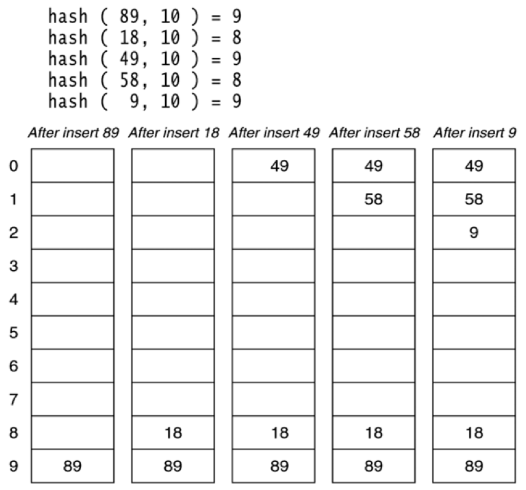
\includegraphics[width=0.5\textwidth,height=\textheight]{images/1.png}
\caption{Linear probing hash table after each insertion. From Weiss,
Figure 20.4}
\end{figure}

\hypertarget{linear-probing-continued}{%
\subsection{Linear Probing (Continued)}\label{linear-probing-continued}}

\begin{itemize}
\tightlist
\item
  How does \passthrough{\lstinline!contains(T t)!} work?

  \begin{itemize}
  \tightlist
  \item
    We'll need to check more than one slot
  \item
    When do we stop and return false?

    \begin{itemize}
    \tightlist
    \item
      As a conservative option, only stop when we've tried all the
      entries in the table
    \item
      As a more efficient option, stop when we hit a
      \passthrough{\lstinline!null!}
    \end{itemize}
  \end{itemize}
\item
  How does \passthrough{\lstinline!remove(T t)!} work?

  \begin{itemize}
  \tightlist
  \item
    Search for the value and set it to \passthrough{\lstinline!null!} if
    it's found

    \begin{itemize}
    \tightlist
    \item
      We can't risk removing it because it could possibly break a search
      chain, as illustrated in the next section
    \end{itemize}
  \end{itemize}
\end{itemize}

\hypertarget{removal-in-open-addressing}{%
\subsection{Removal in Open
Addressing}\label{removal-in-open-addressing}}

\begin{itemize}
\tightlist
\item
  For \passthrough{\lstinline!contains(T t)!} or
  \passthrough{\lstinline!remove(T t)!} we need to follow the implicit
  chain
\item
  Suppose that when we use \passthrough{\lstinline!remove(T t)!}, it
  sets the position the element was in to \passthrough{\lstinline!null!}

  \begin{itemize}
  \item
    If we sue our more efficient method of searching through the hash
    table, assuming linear probing, then we stop our search immediately
    upon hitting the gap that we've introduced.

    This is bad because the value we might want could be directly after
    the gap, if it was put there as the result of a collision.
  \end{itemize}
\end{itemize}

\hypertarget{avoid-breaking-chains}{%
\subsection{Avoid Breaking Chains}\label{avoid-breaking-chains}}

\begin{itemize}
\item
  Don't set the removed records to \passthrough{\lstinline!null!}
\item
  Instead, use place-holders (colloquially called tombstones)
\item
  Example from Weiss:

\begin{lstlisting}[language=Java]
private static class HashEntry {
    public Object element; // the element
    public boolean isActive; // false if marked deleted
    ...
}
\end{lstlisting}

  \begin{itemize}
  \tightlist
  \item
    \passthrough{\lstinline!remove(T t)!} sets
    \passthrough{\lstinline!isActive!} to
    \passthrough{\lstinline!false!}
  \item
    \passthrough{\lstinline!add(T t)!} and
    \passthrough{\lstinline!contains(T t)!} treat inactive slots as
    tombstones
  \item
    \passthrough{\lstinline!rehash()!} ignores inactive entries
  \end{itemize}
\end{itemize}

\hypertarget{linear-probing-implementation}{%
\subsection{Linear Probing
Implementation}\label{linear-probing-implementation}}

\begin{itemize}
\tightlist
\item
  Loop starting from the location

  \begin{itemize}
  \tightlist
  \item
    \passthrough{\lstinline!abs(x.hashCode()) \% tableLength!}
  \end{itemize}
\item
  \passthrough{\lstinline!add(T t)!}

  \begin{itemize}
  \tightlist
  \item
    Loop until we find an empty slot or a tombstone
  \end{itemize}
\item
  \passthrough{\lstinline!contains(T t)!}

  \begin{itemize}
  \tightlist
  \item
    Loop until we find \passthrough{\lstinline!t!} (or fail to do so);
    fail if we hit a \passthrough{\lstinline!null!} or we've tried all
    the entries
  \item
    Finding a tombstone means that we keep searching
  \end{itemize}
\item
  \passthrough{\lstinline!remove(T t)!}

  \begin{itemize}
  \tightlist
  \item
    Loop until we find \passthrough{\lstinline!t!} (or fail to do so);
    fail if we hit a \passthrough{\lstinline!null!} or we've tried all
    the entries
  \item
    Finding a tombstone means that we keep searching
  \item
    If we find \passthrough{\lstinline!t!}, make it a tombstone
  \end{itemize}
\end{itemize}

\hypertarget{linear-probing-issues}{%
\subsection{Linear Probing Issues}\label{linear-probing-issues}}

\begin{itemize}
\tightlist
\item
  Discussion for \passthrough{\lstinline!add(T t)!}

  \begin{itemize}
  \tightlist
  \item
    Adjacent slots get filled first -- that means our hash table suffers
    from primary clustering
  \item
    \textbf{Can \passthrough{\lstinline!add(T t)!} fail?}

    \begin{itemize}
    \tightlist
    \item
      \textbf{Under what conditions?}
    \item
      \textbf{What do we do if it fails?}
    \end{itemize}
  \end{itemize}
\end{itemize}

\hypertarget{linear-probing-load}{%
\subsection{Linear Probing: Load}\label{linear-probing-load}}

\begin{itemize}
\tightlist
\item
  Load has a big effect on performance in linear probing

  \begin{itemize}
  \tightlist
  \item
    The \passthrough{\lstinline!load!} is defined by
    \passthrough{\lstinline!item count / array length!}
  \item
    When the table is nearly full, we end up scanning most of the array
  \item
    The \passthrough{\lstinline!load!} \(\approx I \rightarrow O(n)\)
    for \passthrough{\lstinline!add(T t)!},
    \passthrough{\lstinline!contains(T t)!}, and
    \passthrough{\lstinline!remove(T t)!}
  \end{itemize}
\item
  Theorem

  \begin{itemize}
  \tightlist
  \item
    The average number of cells examined during insertion with linear
    probing is given by
    \[ \frac{1}{2} \left(1 + \frac{1}{(1-load)^2}\right)\]
  \item
    This yields an exceptionally steep exponential growth curve of the
    number of buckets checked for an insertion with respect to the load:
  \end{itemize}
\end{itemize}

\begin{figure}
\centering
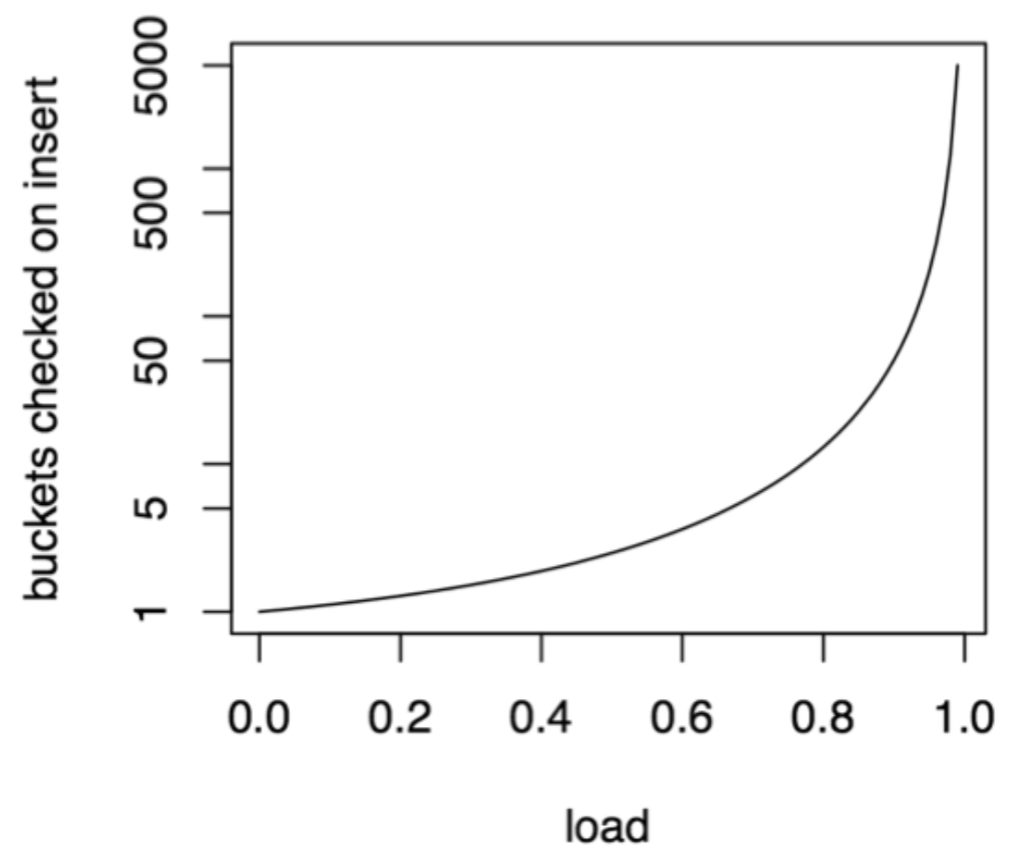
\includegraphics[width=0.5\textwidth,height=\textheight]{images/2.png}
\caption{Number of buckets checked before insertion vs.~load}
\end{figure}

\hypertarget{linear-probing-primary-clustering}{%
\subsection{Linear Probing: Primary
Clustering}\label{linear-probing-primary-clustering}}

\begin{figure}
\centering
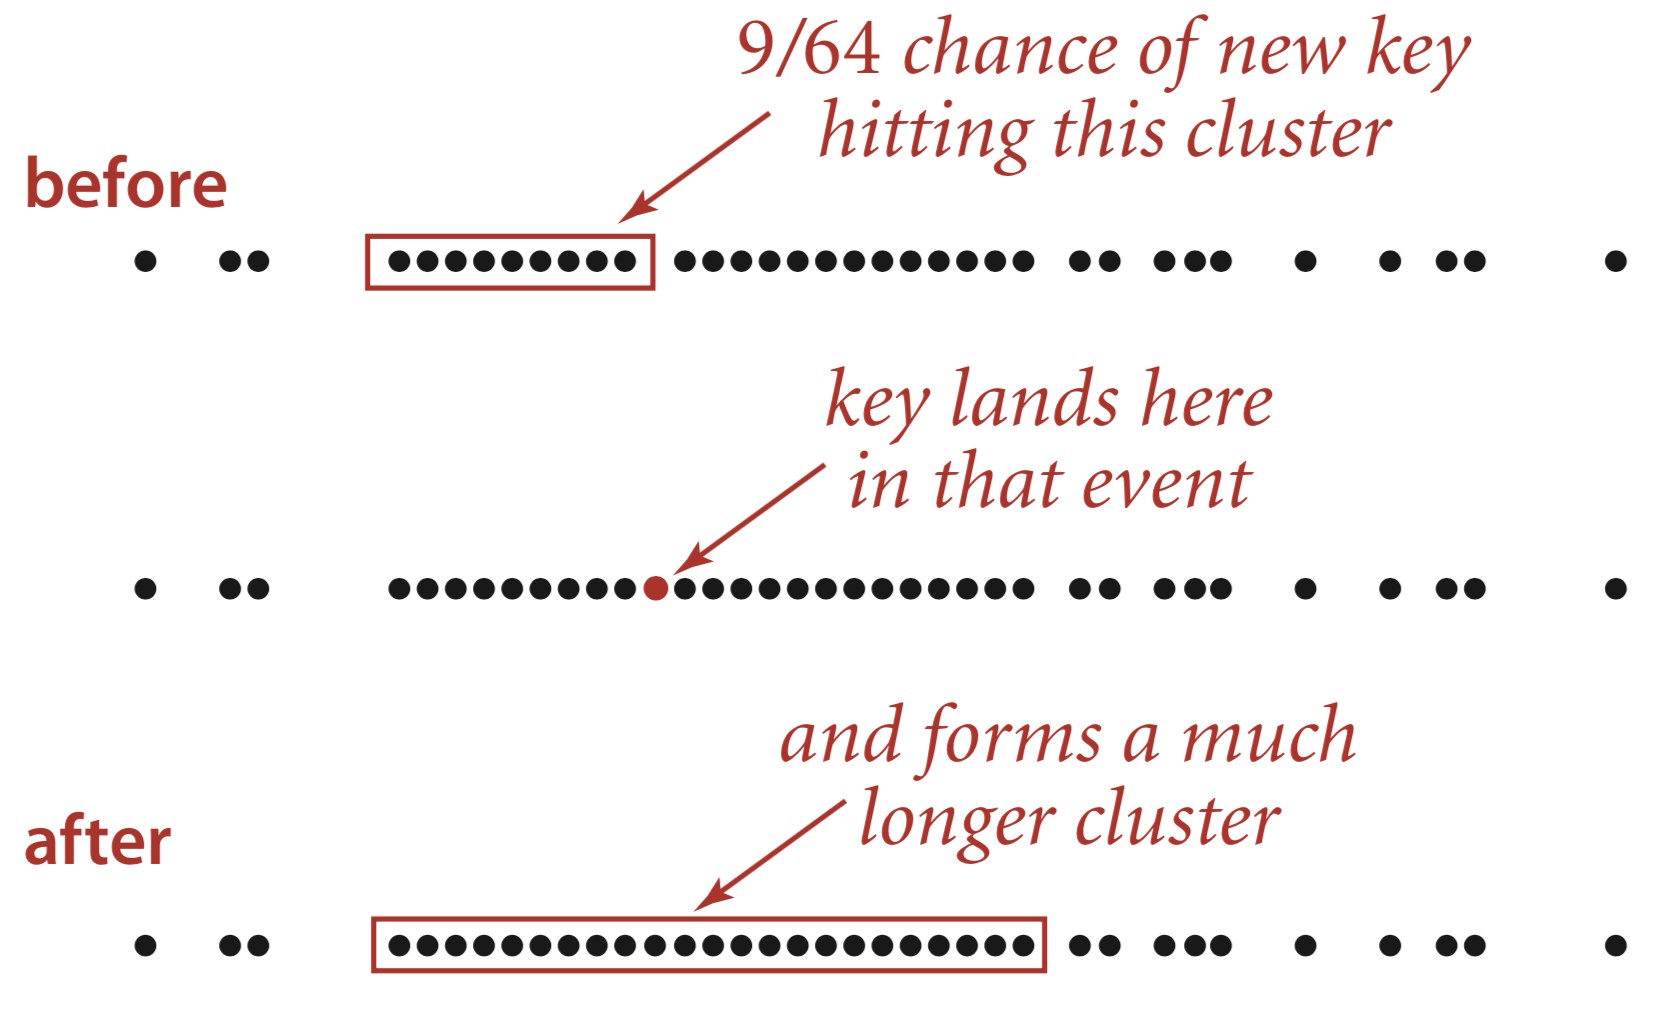
\includegraphics[width=0.5\textwidth,height=\textheight]{images/3.png}
\caption{Clustering in linear probing \((M = 64)\). Sedgewick et. al's
Algorithms, 4th ed.~Chp. 3.4}
\end{figure}

\begin{figure}
\centering
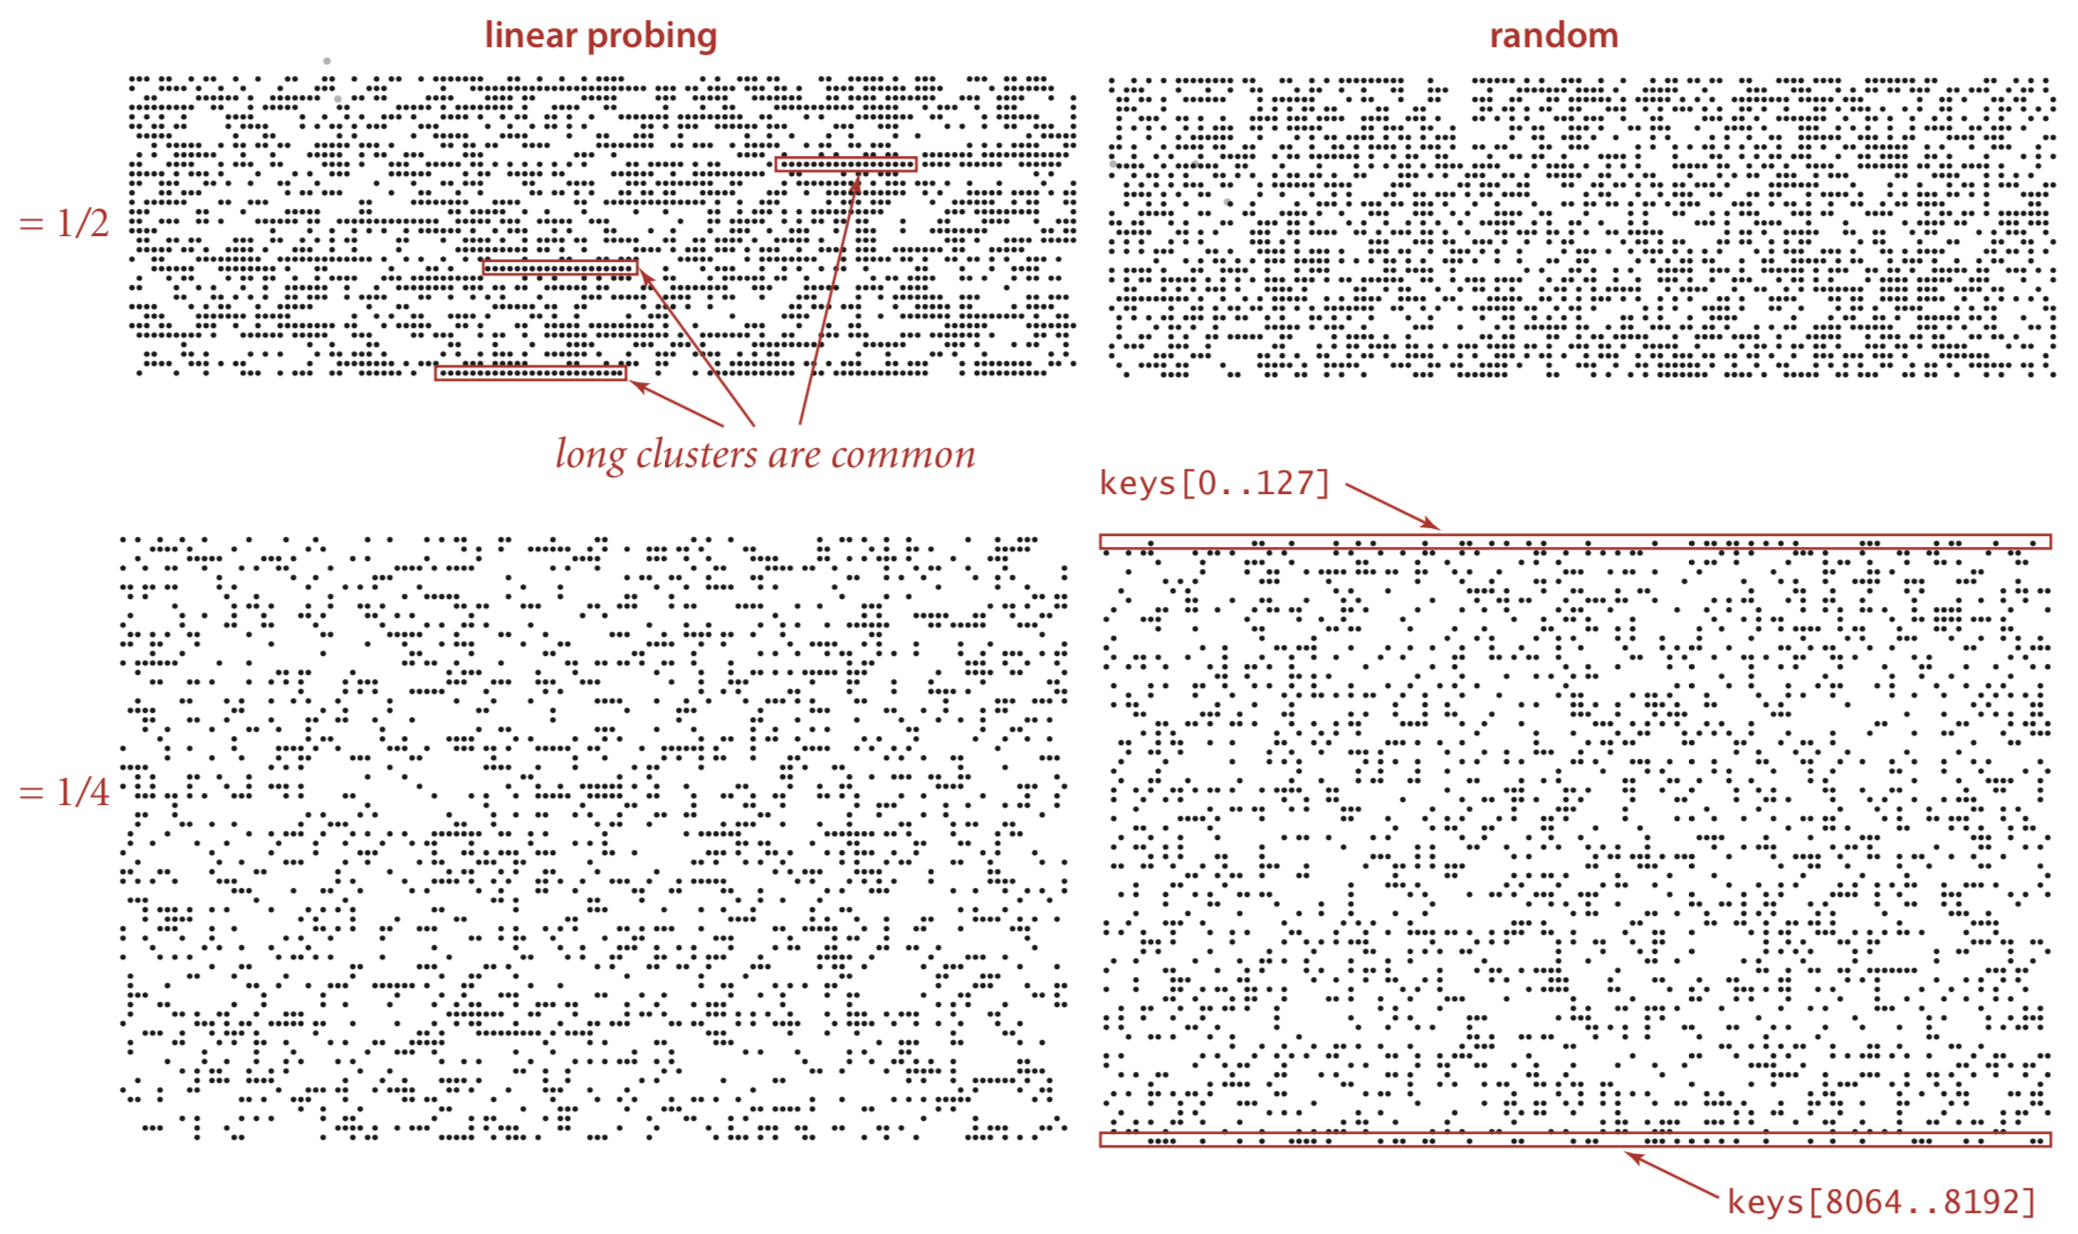
\includegraphics[width=1\textwidth,height=\textheight]{images/4.png}
\caption{Table occupancy patterns (2,048 keys, tables laid out in
128-position rows). Sedgewick et. al's Algorithms, 4th ed.~Chp. 3.4}
\end{figure}

\hypertarget{rehashing}{%
\subsection{Rehashing}\label{rehashing}}

\begin{itemize}
\tightlist
\item
  Rehashing is required for open address hashing

  \begin{itemize}
  \tightlist
  \item
    Tables will get full as we continue to add things to them, creating
    higher penalties for search and insertion
  \item
    Even if the table isn't completely full, an arbitrarily high load
    might warrant a rehashing

    \begin{itemize}
    \tightlist
    \item
      Rehashing means we create a bigger hash table, and copy all of the
      elements over the to the new hash table by recomputing their hash
      code
    \end{itemize}
  \end{itemize}
\item
  We follow a similar procedure for rehashing when we use separate
  chaining

  \begin{itemize}
  \tightlist
  \item
    Allocate a new, larger array (the size should still be prime)
  \item
    Copy over all the active items to the new array

    \begin{itemize}
    \tightlist
    \item
      We'll need to recalculate every item's hash code and re-insert
      them
    \item
      What do we do if we have tombstones?

      \begin{itemize}
      \tightlist
      \item
        We can leave them behind! We only kept them in the first place
        so we didn't break search chains. Since we're essentially
        redoing the entire hash table, we'll develop new search chains
        as we copy the elements over to the new table.
      \end{itemize}
    \end{itemize}
  \end{itemize}
\end{itemize}

\hypertarget{quadratic-probing}{%
\subsection{Quadratic Probing}\label{quadratic-probing}}

\begin{itemize}
\tightlist
\item
  Try the following sequence until an empty array element is found:

  \begin{itemize}
  \tightlist
  \item
    \passthrough{\lstinline!pos!}, \passthrough{\lstinline!pos+1^2!},
    \passthrough{\lstinline!pos+2^2!}, \ldots{}
  \end{itemize}
\item
  Features

  \begin{itemize}
  \tightlist
  \item
    Primary clustering isn't a problem since we're not putting things in
    adjacent cells
  \item
    The complexity of this is \textbf{not} fully understood

    \begin{itemize}
    \tightlist
    \item
      There's no known relation between the load and the average number
      of cells searched
    \item
      It's an interesting open research problem
    \end{itemize}
  \item
    Concerns

    \begin{itemize}
    \tightlist
    \item
      Is it guaranteed to find a spot to add if the table is not full?

      \begin{itemize}
      \tightlist
      \item
        Possibly, yes.
      \end{itemize}
    \item
      Is the exponentiation too expensive to compute?

      \begin{itemize}
      \tightlist
      \item
        Generally, no.
      \end{itemize}
    \end{itemize}
  \end{itemize}
\end{itemize}

\hypertarget{quadratic-probing-example}{%
\subsection{Quadratic Probing Example}\label{quadratic-probing-example}}

\begin{figure}
\centering
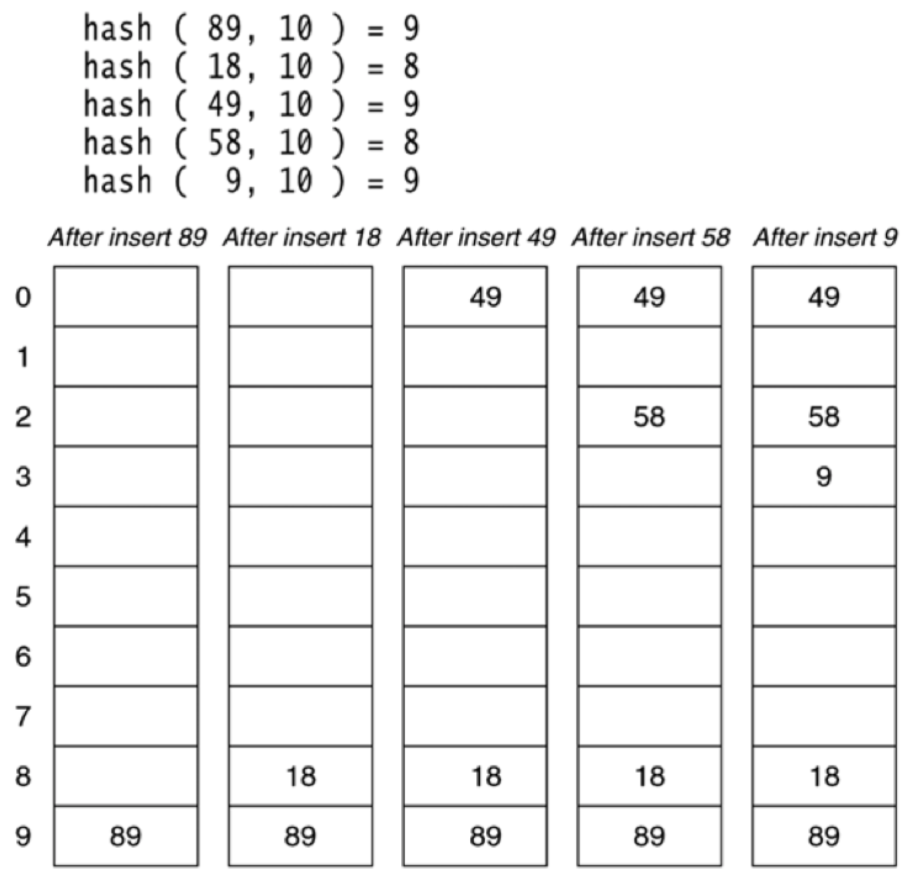
\includegraphics[width=0.5\textwidth,height=\textheight]{images/5.png}
\caption{A quadratic probing hash table after each insertion (note that
the table size was poorly chosen because it is not a prime number).
Weiss, Figure 20.6}
\end{figure}

\hypertarget{issues-with-quadratic-probing}{%
\subsection{Issues with Quadratic
Probing}\label{issues-with-quadratic-probing}}

\begin{itemize}
\item
  As an example, suppose that we have the following table:

  \begin{longtable}[]{cc}
  \toprule
  Index & Contents\tabularnewline
  \midrule
  \endhead
  0 & 48\tabularnewline
  1 &\tabularnewline
  2 & 5\tabularnewline
  3 & 55\tabularnewline
  4 &\tabularnewline
  5 & 40\tabularnewline
  6 & 76\tabularnewline
  \bottomrule
  \end{longtable}

  Assume then that we attempt to do \passthrough{\lstinline!add(47)!}:

  \begin{itemize}
  \tightlist
  \item
    \passthrough{\lstinline!pos = 47 \% 7 = 5!} \(\rightarrow\) fail
  \item
    \passthrough{\lstinline!5 + 12 = 6!} \(\rightarrow\) fail
  \item
    \passthrough{\lstinline!5 + 22 = 9, 9 \% 7 = 2!} \(\rightarrow\)
    fail
  \item
    \passthrough{\lstinline!5 + 32 = 14, 14 \% 7 = 0!} \(\rightarrow\)
    fail
  \item
    \passthrough{\lstinline!5 + 42 = 21, 21 \% 7= 0!} \(\rightarrow\)
    fail
  \item
    \passthrough{\lstinline!5 + 52 = 30, 30 \% 7 = 2!} \(\rightarrow\)
    fail
  \item
    \passthrough{\lstinline!5 + 62 = 41, 41 \% 7 = 6!} \(\rightarrow\)
    fail
  \item
    \passthrough{\lstinline!5 + 72 = 54, 54 \% 7 = 5!} \(\rightarrow\)
    fail
  \item
    This pattern will repeat: \(6, 2, 0, 0, 2, 6, 5, \dots\)
  \item
    We won't be able to \passthrough{\lstinline!add(47)!} even though
    the table isn't full!
  \end{itemize}
\end{itemize}

\hypertarget{quadratic-probing-good-news-everyone}{%
\subsection{Quadratic Probing (Good News
Everyone!)}\label{quadratic-probing-good-news-everyone}}

\begin{itemize}
\tightlist
\item
  We don't have problems as long as the table size is prime \textbf{and}
  the load factor doesn't exceed 0.5 (Weiss, Theorem 20.4, pg 786)

  \begin{itemize}
  \tightlist
  \item
    As long as these premises are held, an item can always be inserted
  \item
    Additionally, we gain the property that no cell is probed twice!
  \end{itemize}
\item
  Quadratic probing can be done efficiently (Weiss, Theorem 20.4, pg
  787)

  \begin{itemize}
  \tightlist
  \item
    Expense operations (like multiplication or exponentiation) can be
    avoided

    \begin{itemize}
    \tightlist
    \item
      As an example, \(H_i = H_{i-1} + 2i - 1 \mod M\)
    \item
      We've gotten rid of the need for exponentiation, and only use
      multiplication by two, which is usually trivially compiled into a
      logical shift
    \end{itemize}
  \end{itemize}
\end{itemize}

\hypertarget{secondary-clustering}{%
\subsection{Secondary Clustering}\label{secondary-clustering}}

\begin{itemize}
\tightlist
\item
  Two values with the same initial position will have the same moves
  while probing
\item
  A popular solution is to use a technique called \emph{double hashing}
\item
  Double hashing:

  \begin{itemize}
  \tightlist
  \item
    The initial position is decided by the first hashing function, as
    usual
  \item
    If the resulting index is occupied, use a second hash function for
    probing

    \begin{itemize}
    \tightlist
    \item
      So instead of checking \passthrough{\lstinline!pos + Hash(x)!},
      \passthrough{\lstinline!pos + 2*Hash(x)!}, and so on, we check
      \passthrough{\lstinline!pos + Hash2(x)!},
      \passthrough{\lstinline!pos + 2*Hash2(x)!}, et al.
    \end{itemize}
  \end{itemize}
\end{itemize}

\hypertarget{double-hashing}{%
\subsection{Double Hashing}\label{double-hashing}}

\begin{itemize}
\tightlist
\item
  The second hash function \(H_2\) can't be zero
\item
  It also should distribute evenly between all the cells
\item
  A common choice:

  \begin{itemize}
  \tightlist
  \item
    \passthrough{\lstinline!Hash(k) = k \% tableSize!}
  \item
    \passthrough{\lstinline!Hash2(k) = (prime - (k \% prime))!}, where
    the prime is less than the size of the table
  \item
    \passthrough{\lstinline!next\_location(i, k) = (Hash(k) + i * Hash2(k)) \% tableSize!}
  \end{itemize}
\end{itemize}

\hypertarget{double-hashing-example}{%
\subsection{Double Hashing Example}\label{double-hashing-example}}

\begin{itemize}
\tightlist
\item
  Given the primary hash function
  \passthrough{\lstinline!Hash(k) = k \% 11!} and the secondary hash
  function \passthrough{\lstinline!Hash2(k) = (7 - (k \% 7))!}:

  \begin{itemize}
  \tightlist
  \item
    \passthrough{\lstinline!add(15)!}

    \begin{itemize}
    \tightlist
    \item
      \passthrough{\lstinline!Hash(15) = 4!}
    \item
      \passthrough{\lstinline!Hash2(15) = 7 - (15 \% 7) = 6!}
    \item
      Sequence for probing is \(4, 10, 5, 0, 6, 1, 7, \dots\)
    \end{itemize}
  \item
    \passthrough{\lstinline!add(26)!}

    \begin{itemize}
    \tightlist
    \item
      \passthrough{\lstinline!Hash(26) = 4!}
    \item
      \passthrough{\lstinline!Hash2(26) = 7 - (26 \% 7) = 2!}
    \item
      Sequence for probing is \(4, 6, 8, 10, 1, 3, 5, \dots\)
    \end{itemize}
  \end{itemize}
\end{itemize}

\hypertarget{hash-table-example}{%
\subsection{Hash Table Example}\label{hash-table-example}}

\begin{figure}
\centering
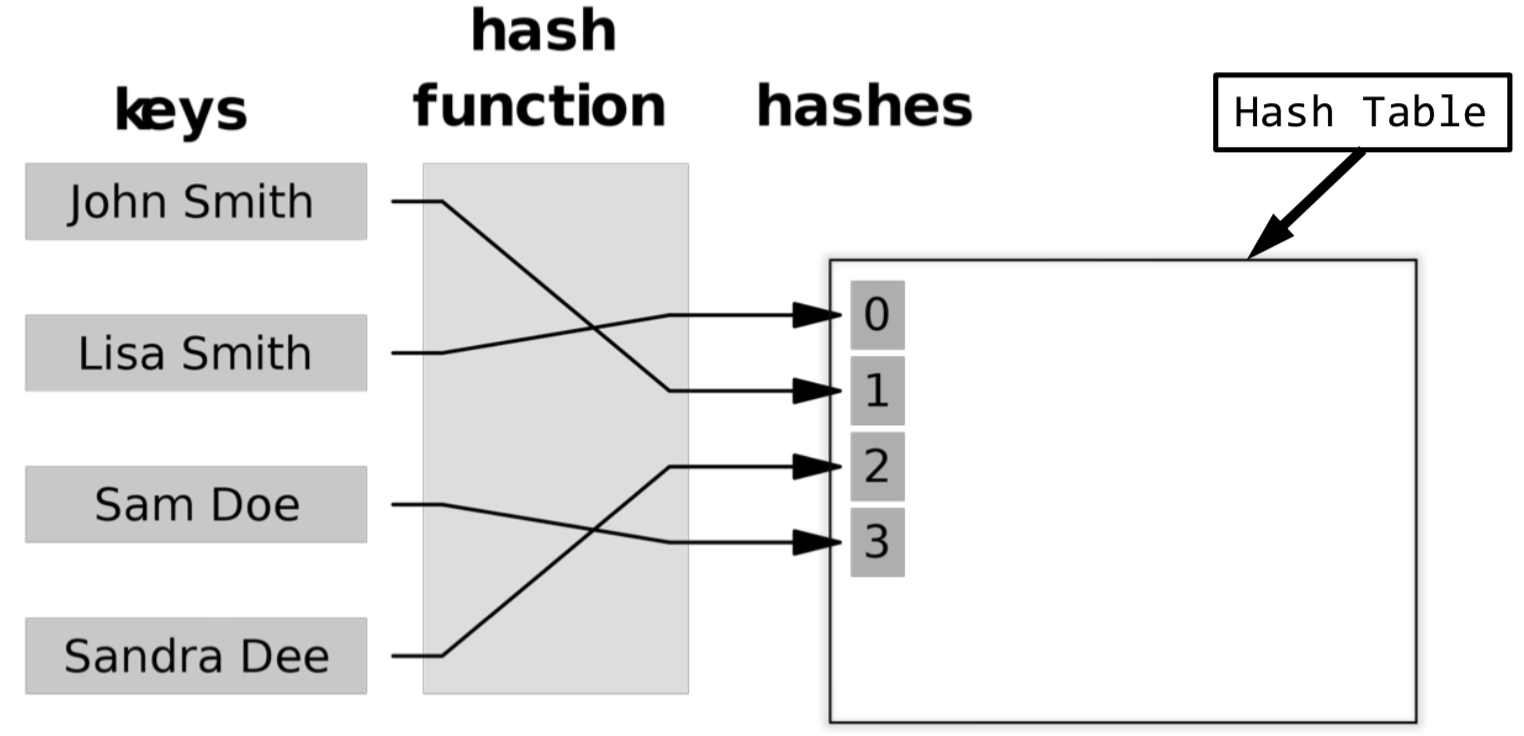
\includegraphics[width=0.5\textwidth,height=\textheight]{images/6.png}
\caption{A hash table without collisions. Retrieved from
\url{https://www.codingeek.com/wp-content/uploads/2017/07/NO-CollisionHash_table_4_1_0_0_0_0_0_LL.svg_.png}}
\end{figure}

\hypertarget{dictionary}{%
\subsection{Dictionary}\label{dictionary}}

\begin{itemize}
\tightlist
\item
  A dictionary defines a mapping between a key and a value

  \begin{itemize}
  \tightlist
  \item
    It can be implemented using a hash table
  \item
    Keys are unique
  \item
    Keys are hashable (their hash code is used to decide where to store
    them)
  \item
    Hash table entries contain the pair
  \end{itemize}
\end{itemize}

\begin{figure}
\centering
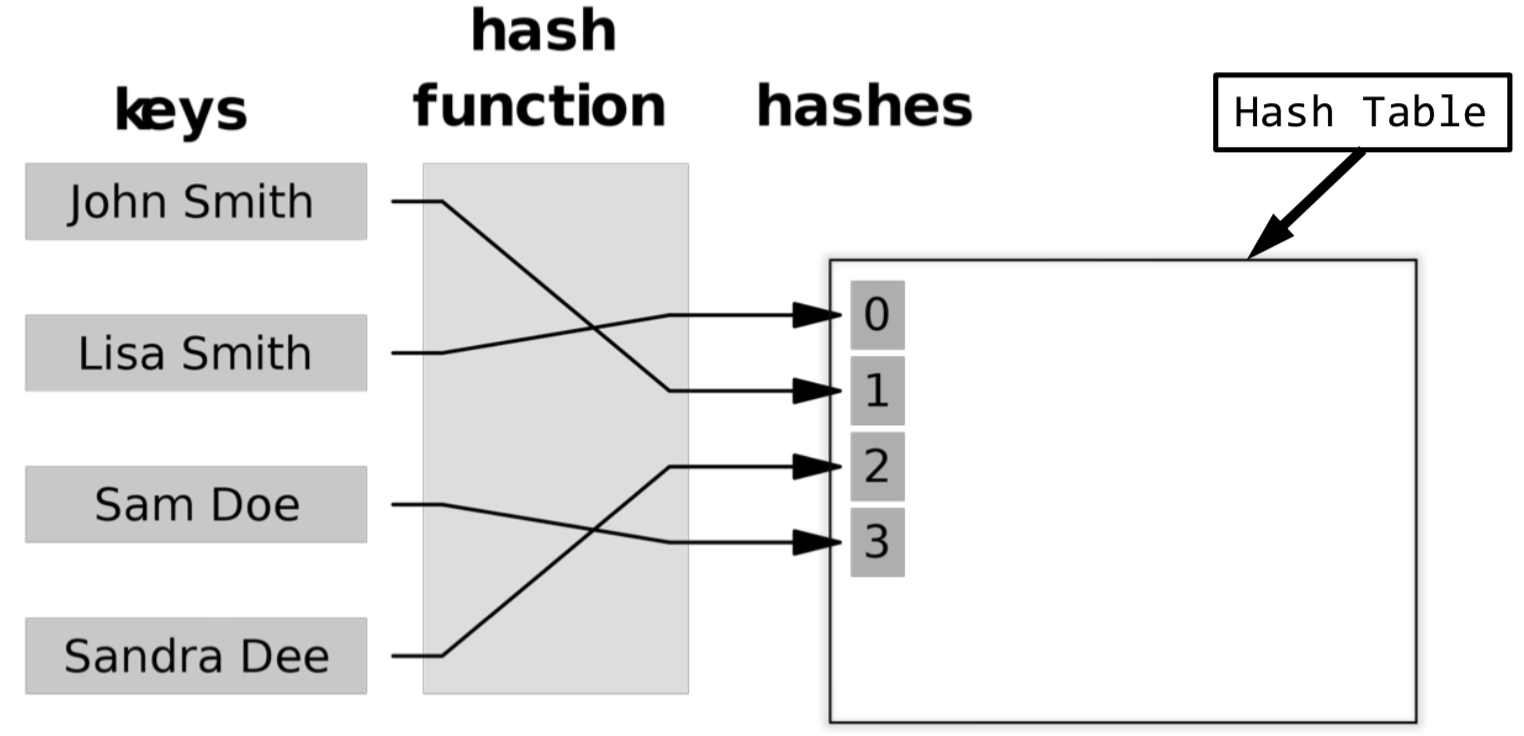
\includegraphics[width=0.5\textwidth,height=\textheight]{images/6.png}
\caption{An example dictionary. Retrieved from
\url{https://upload.wikimedia.org/wikipedia/commons/5/53/Hash_table_lchain_999.svg}}
\end{figure}

\hypertarget{sets-vs.-maps}{%
\subsection{Sets vs.~Maps}\label{sets-vs.-maps}}

\begin{itemize}
\tightlist
\item
  Sets

  \begin{itemize}
  \tightlist
  \item
    Just like the mathematical set\ldots{} except it can't be infinite
    (which is a bummer)
  \item
    Unordered collection of items
  \item
    No duplicates allowed
  \end{itemize}
\item
  Maps

  \begin{itemize}
  \tightlist
  \item
    Essentially some relation \(M\) defined by \(M\subset K \times V\)
    where \(K\) is the set of keys, and \(V\) is the \textbf{list} of
    values (the values are not necessarily unique).
  \item
    Each key maps to a value

    \begin{itemize}
    \tightlist
    \item
      As an example, the key \passthrough{\lstinline!"G00123123"!} might
      map to \passthrough{\lstinline!"Sam Samson"!}
    \end{itemize}
  \item
    Python dictionaries are maps
  \end{itemize}
\item
  Both are usually implemented with a hash table

  \begin{itemize}
  \tightlist
  \item
    We can typically implement them with normal lists, ordered or
    unordered
  \end{itemize}
\end{itemize}

\hypertarget{operations-on-sets-or-maps}{%
\subsection{Operations on Sets or
Maps}\label{operations-on-sets-or-maps}}

\hypertarget{sets}{%
\subsubsection{Sets}\label{sets}}

\begin{itemize}
\tightlist
\item
  \passthrough{\lstinline!add(T t)!}: add the value to the set if it's
  not in the set yet
\item
  \passthrough{\lstinline!remove(T t)!}: remove the value from the set
\item
  \passthrough{\lstinline!has(T t)!}: find out if the value is contained
  in the set
\end{itemize}

\hypertarget{maps}{%
\subsubsection{Maps}\label{maps}}

\begin{itemize}
\tightlist
\item
  \passthrough{\lstinline!put(K k, V v)!}: puts the value
  \passthrough{\lstinline!v!} at the key \passthrough{\lstinline!k!}'s
  location
\item
  \passthrough{\lstinline!remove(K k)!}: remove the value associated
  with the given key
\item
  \passthrough{\lstinline!has(K k)!}: find out if the key is contained
  in the set of keys
\item
  \passthrough{\lstinline!get(K k)!}: get the value associated with the
  given key
\end{itemize}

\hypertarget{implementation}{%
\subsection{Implementation}\label{implementation}}

\begin{itemize}
\tightlist
\item
  You can build a \passthrough{\lstinline!Set!} out of a
  \passthrough{\lstinline!Map!}

  \begin{itemize}
  \tightlist
  \item
    We really only need a hash table that does not allow duplicates
  \item
    We don't actually need a pair of keys and values

    \begin{itemize}
    \tightlist
    \item
      We can keep the value and key to be the same;
    \item
      Or we can use only the key, and have the values be null
    \end{itemize}
  \end{itemize}
\item
  Examples:

  \begin{itemize}
  \tightlist
  \item
    Java's own \passthrough{\lstinline!HashSet!}
  \item
    Weiss 6.7.2
  \end{itemize}
\item
  You can also build a \passthrough{\lstinline!Map!} out of a
  \passthrough{\lstinline!Set!}

  \begin{itemize}
  \tightlist
  \item
    We get \passthrough{\lstinline!add(T t)!},
    \passthrough{\lstinline!remove(T t)!}, and
    \passthrough{\lstinline!has(T t)!} for free
  \item
    We can construct a set with items as a pair of keys and values
  \item
    We need to support \passthrough{\lstinline!has(K k)!},
    \passthrough{\lstinline!get(K k)!},
    \passthrough{\lstinline!remove(K k)!}, and
    \passthrough{\lstinline!put(K k, V v)!}

    \begin{itemize}
    \tightlist
    \item
      Keys need to be unique, so we'll have to ensure that property
      holds
    \end{itemize}
  \item
    Essentially we need to compare and / or hash items based only on
    their key

    \begin{itemize}
    \tightlist
    \item
      \emph{Key-Value pairs are thus said to be equal if their keys are
      equal}
    \end{itemize}
  \item
    See Weiss 6.8 for more
  \end{itemize}
\end{itemize}

\hypertarget{hashing-summary}{%
\subsection{Hashing Summary}\label{hashing-summary}}

\begin{itemize}
\tightlist
\item
  Hash tables provide \(O(1)\) \passthrough{\lstinline!add(T t)!},
  \passthrough{\lstinline!remove(T t)!}, and
  \passthrough{\lstinline!contains(T t)!}
\item
  Hashing functions compute hash codes

  \begin{itemize}
  \tightlist
  \item
    They must be easy to compute
  \item
    They must distribute well
  \item
    And the \emph{should} make use of prime numbers
  \end{itemize}
\item
  Hash collisions can be mitigated with:

  \begin{itemize}
  \tightlist
  \item
    Separate chaining

    \begin{itemize}
    \tightlist
    \item
      in which each hash bucket is a list
    \end{itemize}
  \item
    Or in open address hashing

    \begin{itemize}
    \tightlist
    \item
      Where we look at buckets using some sequence

      \begin{itemize}
      \tightlist
      \item
        Either in a linear or quadratic fashion, or by using double
        hashing
      \end{itemize}
    \end{itemize}
  \end{itemize}
\end{itemize}

\hypertarget{hash-table-big-o}{%
\subsection{Hash Table Big-O}\label{hash-table-big-o}}

\begin{longtable}[]{cccccc}
\toprule
Approaches & Cases & \passthrough{\lstinline!add(T t)!}\(^*\) &
\passthrough{\lstinline!has(T t)!} &
\passthrough{\lstinline!remove(T t)!} & iterate\tabularnewline
\midrule
\endhead
Separate Chaining & Average & \(O(n/m)\) & \(O(n/m)\) & \(O(n/m)\) &
\(O(n+m)\)\tabularnewline
& Worst & \(O(n)\) & \(O(n)\) & \(O(n)\) & \(O(n+m)\)\tabularnewline
Open Addressing & Average\(^{**}\) & \(O(1)\) & \(O(1)\) & \(O(1)\) &
\(O(m)\)\tabularnewline
& Worst & \(O(n)\) & \(O(n)\) & \(O(n)\) & \(O(m)\)\tabularnewline
\bottomrule
\end{longtable}

\begin{itemize}
\tightlist
\item
  \(n\): the number of values in the hash table
\item
  \(m\): the number of entries (the array capacity)
\item
  \(^*\): assumes no duplicates are allowed, and does not consider
  rehash overhead
\item
  \(^{**}\): if load is low and a good hash function is used
\end{itemize}

\hypertarget{next-lecture}{%
\subsection{Next Lecture}\label{next-lecture}}

\begin{itemize}
\tightlist
\item
  Project 3

  \begin{itemize}
  \tightlist
  \item
    Binary search tree
  \end{itemize}
\item
  Topic: Graphs

  \begin{itemize}
  \tightlist
  \item
    Reading: Chapter 14
  \end{itemize}
\end{itemize}

\end{document}
